\chapter{Methodology}

\section{Overview}

This chapter presents a comprehensive methodology for predicting Antimicrobial Resistance (AMR) using machine learning techniques applied to resistance gene profiles. The proposed approach demonstrates that resistance gene-based prediction can achieve performance comparable to, or exceeding, whole-genome sequence (WGS)-based methods while maintaining computational efficiency and biological interpretability. 

The methodology includes six major stages:

\begin{enumerate}
    \item Dataset Collection and Preprocessing
    \item Feature Engineering
    \item Feature Selection
    \item Class Imbalance Handling
    \item Model Training and Ensemble Construction
    \item Model Interpretability and Explainability
\end{enumerate}

The pipeline addresses challenges inherent in AMR genomic data such as high dimensionality, extreme sparsity, and class imbalance. Figure~\ref{fig:pipeline} illustrates the overall workflow.

\begin{figure}[h]
\centering
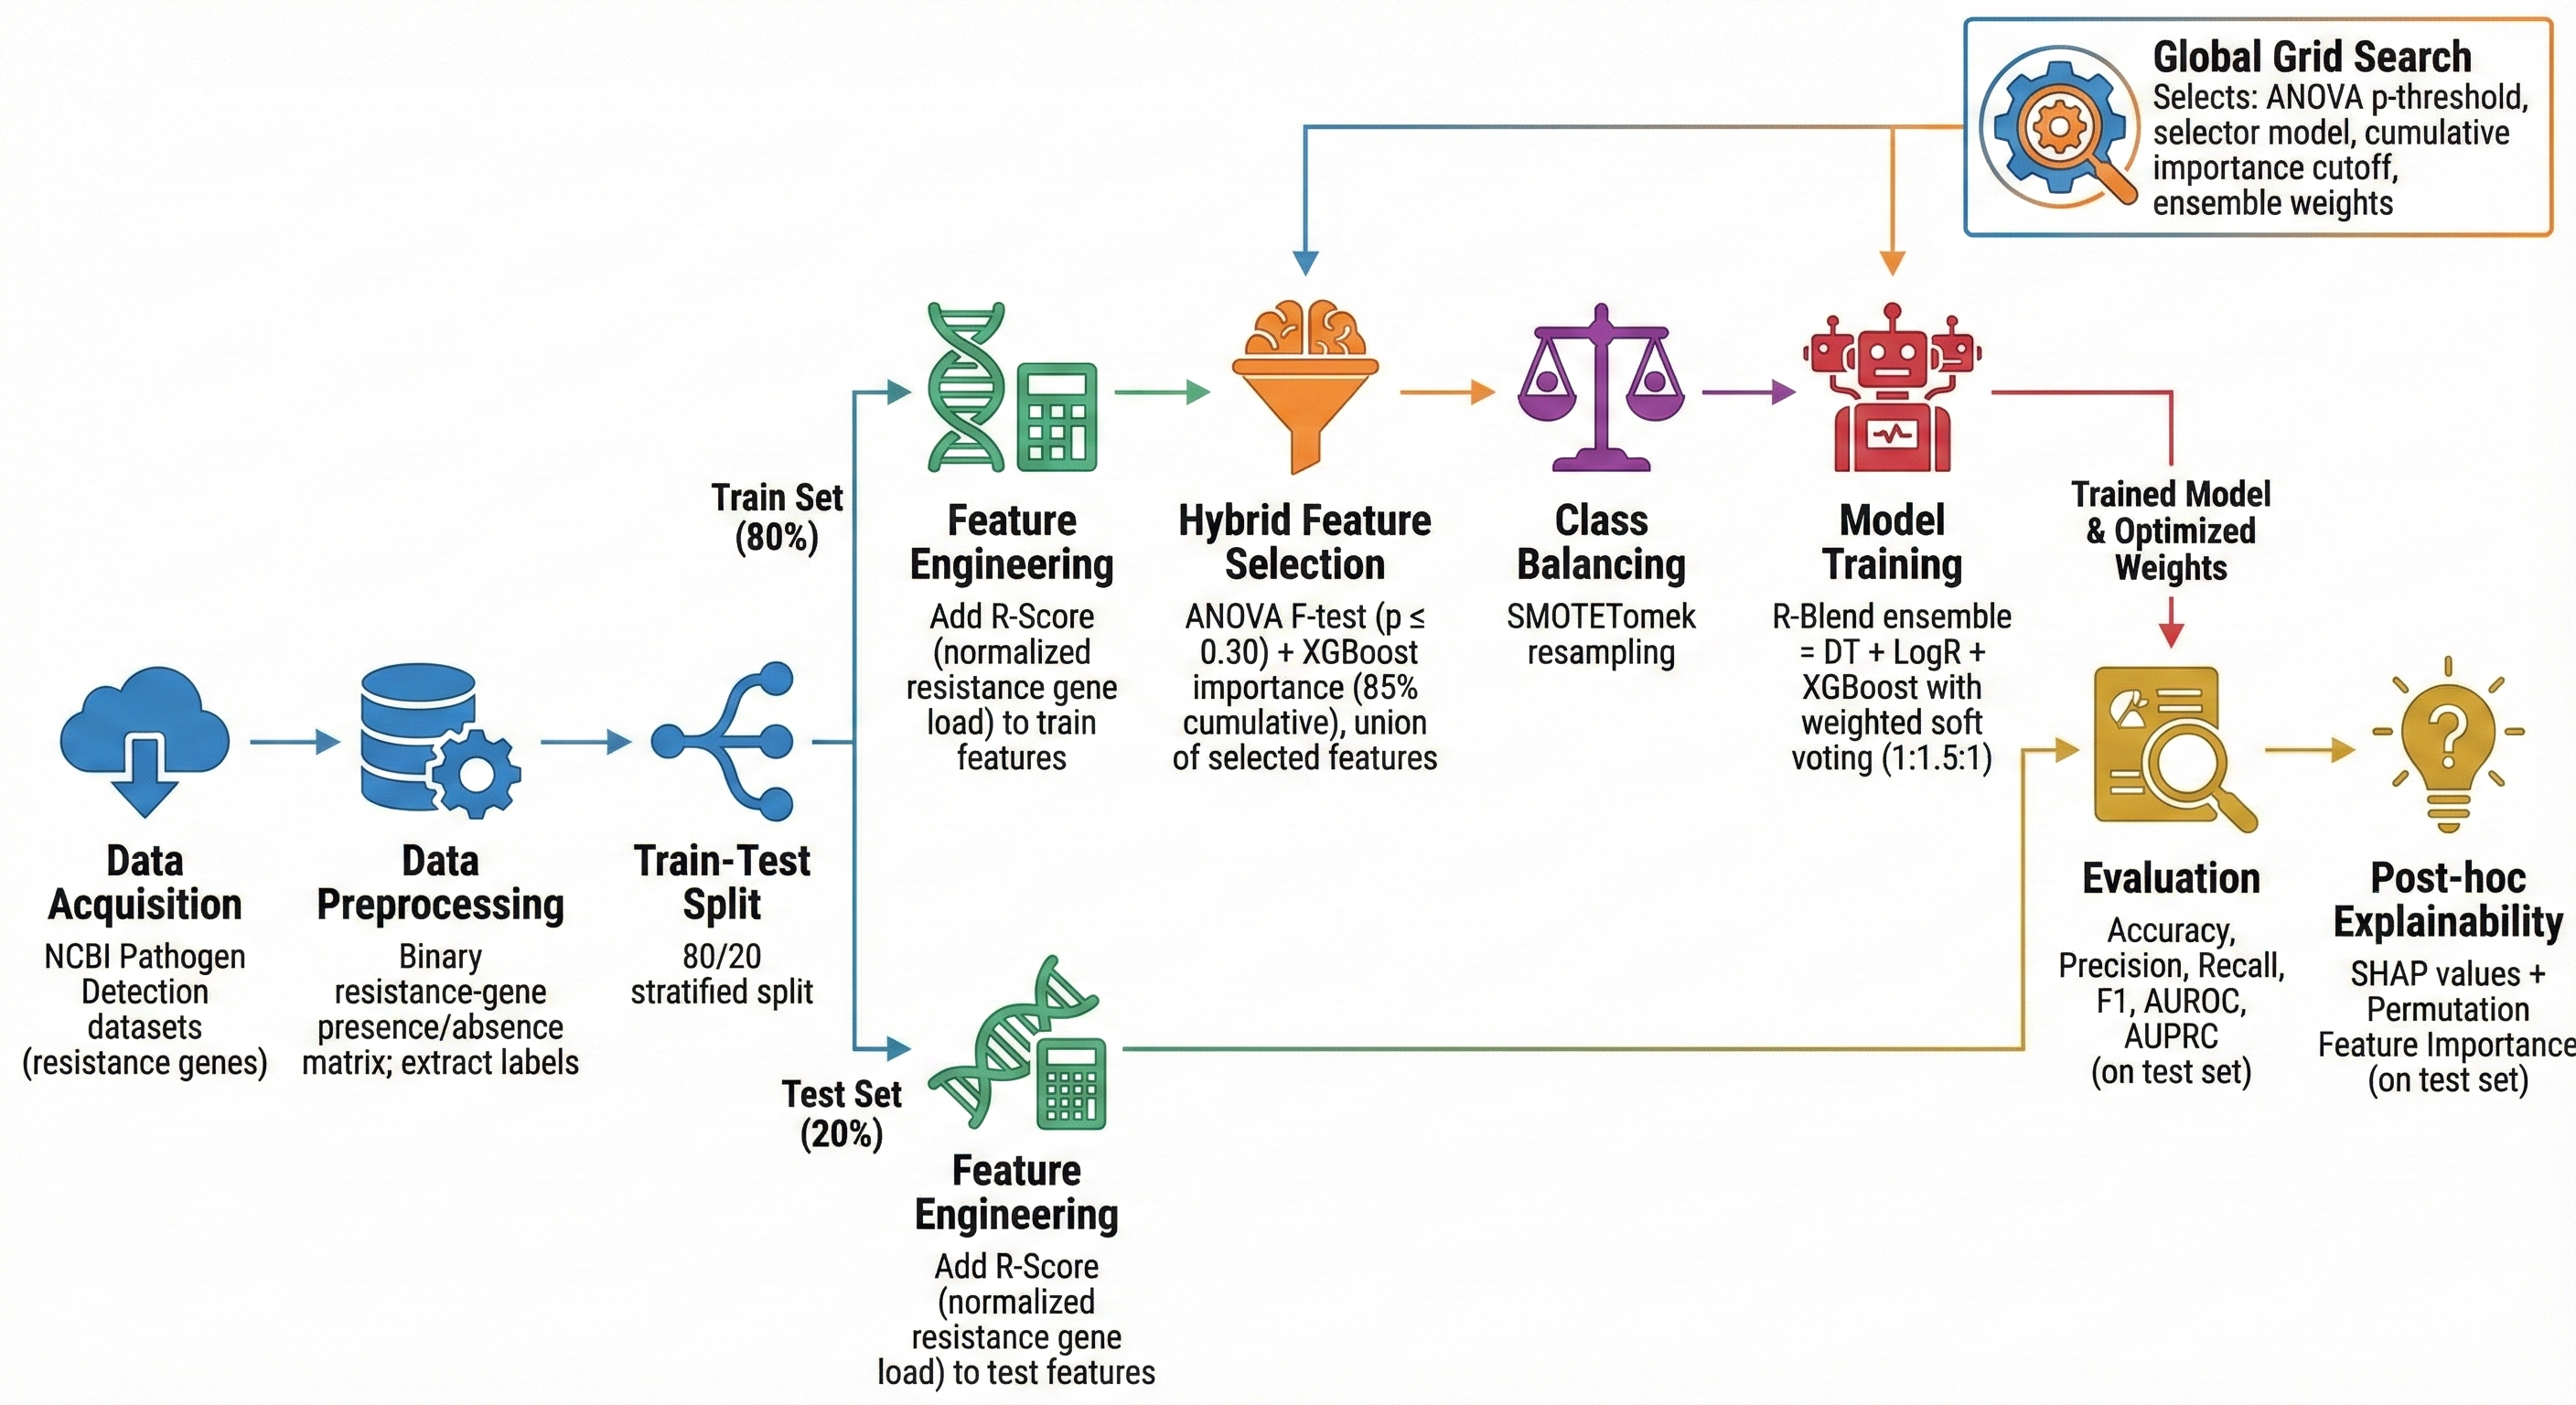
\includegraphics[width=0.95\textwidth]{figures/Workflow Diagram.png}
\caption{End-to-end AMR prediction pipeline of the proposed method}
\label{fig:pipeline}
\end{figure}

\section{Dataset Collection and Preprocessing}

\subsection{Dataset Description}

Unlike prior works that focus on a single antibiotic--pathogen pair, our study analyzes 12 AMR datasets from Sunuwar et al.~\cite{sunuwar2021}, each representing a unique antibiotic--pathogen combination. To benchmark against WGS-based methods, we also used the dataset from Noman et al.~\cite{noman2023}, which includes whole-genome sequences of \textit{Pseudomonas aeruginosa} isolates.

\subsection{Resistance Gene-Based Datasets (Sunuwar et al.)}

The first 12 datasets were collected from the NCBI Pathogen Detection portal and curated by Sunuwar et al. Each dataset contains resistance gene presence/absence information and phenotypic AMR labels across several pathogens and antibiotics:

\begin{itemize}
    \item \textbf{K. pneumoniae (KN)}: Doripenem, Ertapenem, Imipenem, Meropenem  
    \item \textbf{E. coli/Shigella (ECS)}: Doripenem, Ertapenem, Imipenem, Meropenem  
    \item \textbf{P. aeruginosa (PA)}: Doripenem  
    \item \textbf{S. enterica (SE)}: Streptomycin, Kanamycin  
    \item \textbf{C. jejuni (CJ)}: Clindamycin  
\end{itemize}

These datasets vary widely in sample size (26--1042 isolates), feature count (11--326 genes), and class distribution.

\begin{table}[h]
\centering
\caption{Summary of the 12 resistance gene-based datasets}
\begin{tabular}{l c c c c}
\hline
Dataset & Isolates & Genes & Resistant & Susceptible \\
\hline
Doripenem (KN) & 316 & 325 & 241 & 75 \\
Ertapenem (KN) & 181 & 324 & 90 & 91 \\
Meropenem (ECS) & 91 & 236 & 45 & 46 \\
Ertapenem (ECS) & 129 & 236 & 61 & 68 \\
Doripenem (ECS) & 49 & 236 & 25 & 24 \\
Imipenem (ECS) & 64 & 236 & 37 & 27 \\
Doripenem (PA) & 44 & 164 & 22 & 22 \\
Streptomycin (SE) & 1042 & 179 & 542 & 500 \\
Imipenem (KN) & 200 & 324 & 113 & 87 \\
Clindamycin (CJ) & 26 & 43 & 8 & 18 \\
Meropenem (KN) & 238 & 324 & 106 & 132 \\
Kanamycin (SE) & 991 & 179 & 493 & 498 \\
\hline
\end{tabular}
\end{table}

Figure~\ref{fig:classdist} shows the class imbalance characteristics.

\begin{figure}[h]
\centering
\includegraphics[width=0.9\textwidth]{figures/figure3_2_2.png}
\caption{Class distribution across antibiotic--pathogen datasets}
\label{fig:classdist}
\end{figure}

\subsection{WGS-Based Dataset (Noman et al.)}

To compare resistance gene-based and WGS-based AMR prediction, we used the dataset from Noman et al.~\cite{noman2023}, consisting of 1437 \textit{P. aeruginosa} isolates annotated with phenotypic resistance against 12 antibiotics.

\begin{table}[h]
\centering
\caption{Summary of Noman et al. WGS-based dataset}
\begin{tabular}{l c c c}
\hline
Drug & Isolates & Resistant & Susceptible \\
\hline
Ampicillin & 1437 & 1428 & 9 \\
Amoxicillin & 1437 & 1423 & 14 \\
Meropenem & 1437 & 814 & 623 \\
Cefepime & 1437 & 1415 & 22 \\
Fosfomycin & 1437 & 1425 & 12 \\
Ceftazidime & 1437 & 1428 & 9 \\
Chloramphenicol & 1437 & 1405 & 32 \\
Erythromycin & 1437 & 36 & 1401 \\
Tetracycline & 1437 & 205 & 1232 \\
Gentamycin & 1437 & 608 & 829 \\
Butirosin & 1437 & 30 & 1407 \\
Ciprofloxacin & 1437 & 1020 & 417 \\
\hline
\end{tabular}
\end{table}

\subsection{Binary Gene Matrix Construction}

Each dataset was converted into a binary gene presence/absence matrix:

\[
x_{i,j} = 
\begin{cases}
1, & \text{if gene } g_j \text{ is present in isolate } i \\
0, & \text{otherwise}
\end{cases}
\]

Gene completeness categories (COMPLETE, PARTIAL, PARTIAL\_END\_OF\_CONTIG) were encoded as additional binary features.  
The target variable was:

\[
y = 
\begin{cases}
1 & \text{Resistant} \\
0 & \text{Susceptible}
\end{cases}
\]

\section{Feature Engineering}

\subsection{Resistance Gene Load Score (R-Score)}

A novel engineered feature capturing cumulative gene burden:

\[
\text{R-Score}_i = \sum_{j=1}^n x_{i,j}
\]

Normalized using Min-Max scaling:

\[
\text{R-Score}'_i = \frac{\text{R-Score}_i - \min(\text{R-Score})}{\max(\text{R-Score}) - \min(\text{R-Score})}
\]

R-Score consistently improved prediction performance and separated resistant vs. susceptible classes.

\section{Feature Selection}

AMR gene datasets are high-dimensional and sparse. We adopt a hybrid, two-stage feature selection approach.

\subsection{Stage 1: ANOVA F-test}

The ANOVA F-statistic measures linear discriminative power:

\[
F(g_j) = \frac{\text{Between-class variance}}{\text{Within-class variance}}
\]

Features with p-value $\le$ 0.30 were retained. R-Score was always retained.

\subsection{Stage 2: XGBoost Embedded Importance}

An XGBoost classifier was trained (400 trees, depth 6), and features were ranked by importance.  
Features contributing to the top 85\% cumulative importance were selected:

\[
S_{\text{XGB}} = \{ g_j : \sum \text{Importance}(g_j) \le 0.85 \}
\]

\subsection{Union-Based Integration}

Final feature set:

\[
S_{\text{final}} = S_{\text{ANOVA}} \cup S_{\text{XGB}}
\]

This union preserved features useful for both linear and nonlinear decision boundaries.

\section{Class Imbalance Handling}

\subsection{Resampling Alternatives Evaluated}

\begin{itemize}
    \item Random Oversampling  
    \item Random Undersampling  
    \item SMOTE  
    \item ADASYN  
    \item Borderline-SMOTE  
    \item SMOTE-ENN  
    \item SMOTE-Tomek  
\end{itemize}

\subsection{Selected Method: SMOTETomek}

SMOTETomek combines SMOTE oversampling with Tomek links removal.

Benefits for AMR gene matrices:

\begin{itemize}
    \item Removes ambiguous samples at class boundaries  
    \item Avoids unrealistic synthetic gene profiles  
    \item Reduces overfitting  
    \item Produces cleaner linear separability  
\end{itemize}

Applied \textbf{only to training data} after feature selection.

\section{Model Training and Ensemble Construction}

\subsection{Base Models Evaluated}

\begin{itemize}
    \item Logistic Regression (LogR)
    \item Support Vector Machine (SVM, RBF kernel)
    \item Decision Tree (DT)
    \item Random Forest (RF)
    \item XGBoost (XGB)
\end{itemize}

\subsection{R-Blend Ensemble}

A weighted soft-voting ensemble combining:

\begin{itemize}
    \item DT (weight = 1.0)
    \item LogR (weight = 1.5)
    \item XGB (weight = 1.0)
\end{itemize}

Soft voting probability:

\[
P(y=c|x) = \frac{\sum_i w_i \, P_i(y=c|x)}{\sum_i w_i}
\]

LogR weight is higher due to better calibration and linear separability after feature engineering.

\subsection{Training Protocol}

\begin{itemize}
    \item 80/20 stratified split  
    \item Feature selection on training data only  
    \item SMOTETomek applied to training data only  
    \item 5-fold cross-validation  
    \item Random seed = 42  
\end{itemize}

\section{Evaluation Metrics}

Given the severe clinical consequences of misclassifying resistant isolates, recall is prioritized.

\subsection{Metric Priority}

\begin{enumerate}
    \item \textbf{Recall (Sensitivity)} — most important clinically  
    \item \textbf{F1-score} — primary publication metric  
    \item AUROC  
    \item AUPRC  
    \item Precision  
    \item Accuracy (not emphasized due to imbalance)  
\end{enumerate}

\subsection{Metric Definitions}

\[
\text{Accuracy} = \frac{TP + TN}{TP + TN + FP + FN}
\]

\[
\text{Precision} = \frac{TP}{TP + FP}
\]

\[
\text{Recall} = \frac{TP}{TP + FN}
\]

\[
\text{F1} = \frac{2\,(\text{Precision}\times\text{Recall})}{\text{Precision}+\text{Recall}}
\]

\section{Model Interpretability and Explainability}

\subsection{Permutation Importance}

\[
\text{Importance}(g_j) = \text{Perf}_{\text{original}} - \text{Perf}_{\text{shuffled}(g_j)}
\]

\subsection{SHAP Explanations}

Model output:

\[
f(x) = \phi_0 + \sum_j \phi_j(x)
\]

TreeExplainer and LinearExplainer were used for XGB/DT and LogR models, respectively.

\subsection{Ensemble SHAP}

\[
\phi_{j,\text{ensemble}}(x) = \frac{\sum_i w_i \phi_{j,i}(x)}{\sum_i w_i}
\]

\section{Experimental Design and Validation}

\subsection{Ablation Studies}

We evaluated the impact of:

\begin{itemize}
    \item Removing R-Score  
    \item Changing resampling strategy  
    \item Using individual base models vs. R-Blend  
    \item Alternative feature selection configurations  
\end{itemize}

\subsection{Cross-Dataset Generalization}

The full pipeline was applied independently to all 12 datasets (80/20 split). Average metrics were computed across datasets.

\subsection{Comparative Analysis}

Benchmarked against:

\begin{itemize}
    \item Sunuwar \& Azad (gene-based baseline)  
    \item Noman et al. (WGS-based BioWeka framework)  
\end{itemize}

\section{Implementation Details}

The pipeline was implemented in Python 3.x using:

\begin{itemize}
    \item \texttt{scikit-learn}
    \item \texttt{XGBoost}
    \item \texttt{imbalanced-learn}
    \item \texttt{SHAP}
    \item \texttt{pandas}, \texttt{NumPy}
\end{itemize}

Experiments ran on Google Colab with GPU support.

\section{Chapter Summary}

This chapter detailed the complete methodology for AMR prediction using resistance gene profiles, including R-Score feature engineering, hybrid ANOVA--XGBoost feature selection, SMOTETomek resampling, R-Blend ensemble learning, and model interpretability through SHAP and permutation importance. The next chapter presents the experimental results.

